% =====================================================================
% CVGIP 2026 Full Paper
% Unsupervised Deep Clustering for Insect Monitoring on Sticky Traps
% in Melon Greenhouses with DINOv2 and Hierarchical Sub-clustering
% Compile with: pdflatex (or xelatex / lualatex)
% =====================================================================
\documentclass[10pt,a4paper,twocolumn]{article}

% ---------- Page geometry (CVGIP 2026 template) ----------
% Print area: 175mm x 226mm; top margin 25mm, left margin 19mm,
% column width 83mm, column gap 8mm.
\usepackage[a4paper,
            top=25mm, left=19mm, right=19mm, bottom=25mm,
            columnsep=8mm]{geometry}

% ---------- Font (Times New Roman family) ----------
\usepackage{times}
\usepackage[T1]{fontenc}
\usepackage[utf8]{inputenc}

% ---------- Common packages ----------
\usepackage{graphicx}
\usepackage{booktabs}
\usepackage{array}
\usepackage{amsmath,amssymb}
\usepackage{caption}
\usepackage{url}
\usepackage{hyperref}
\usepackage{titlesec}
\usepackage{enumitem}
\usepackage{authblk}

% ---------- Section style: "1. INTRODUCTION" (centered, ALL CAPS, bold) ----------
\titleformat{\section}
  {\centering\normalfont\bfseries\uppercase}
  {\thesection.}{0.5em}{}
% Subsection: "1.1. Title" (left, initial caps, bold)
\titleformat{\subsection}
  {\normalfont\bfseries}
  {\thesubsection.}{0.5em}{}
\titleformat{\subsubsection}
  {\normalfont\bfseries\itshape}
  {\thesubsubsection.}{0.5em}{}

% ---------- No first-paragraph indent inside sections ----------
\usepackage{indentfirst}
\setlength{\parindent}{1.5em}

% ---------- Captions: "Fig. 1." / "Table 1." ----------
\captionsetup[figure]{labelfont=bf, labelsep=period, name=Fig.}
\captionsetup[table]{labelfont=bf, labelsep=period, name=Table}

% ---------- Title block ----------
\title{\fontsize{14pt}{16pt}\selectfont\bfseries
UNSUPERVISED DEEP CLUSTERING FOR INSECT MONITORING ON STICKY TRAPS IN MELON GREENHOUSES WITH DINOv2 AND HIERARCHICAL SUB-CLUSTERING}

\author[1]{Author One}
\author[1]{Author Two}
\author[2]{Author Three}
\affil[1]{Department of XXX, XXX University}
\affil[2]{XXX Research Institute}
\affil[ ]{\texttt{\{author1, author2\}@xxx.edu.tw}}

\date{}

% =====================================================================
\begin{document}
\twocolumn[
  \begin{@twocolumnfalse}
    \maketitle
    \begin{abstract}
\noindent
Yellow sticky traps are a standard tool for monitoring flying pests in greenhouse agriculture, but counting and identifying the trapped insects is still performed manually, which is slow, fatiguing, and difficult to scale across a whole farm. Supervised detectors can automate this task, yet they require large, expert-annotated datasets that are costly to obtain for the many morphologically similar species found on a single trap. We present a fully unsupervised pipeline that takes raw sticky-trap photographs and groups the individual insects with no human labels. The pipeline first isolates each insect through border cropping, corner masking, and an adaptive-tiling step driven by HSV background detection. It then learns visual representations with Stable Cluster Discrimination (SeCu) built on a frozen DINOv2 backbone, which we extend with medoid-based center re-estimation and a graph-modularity loss (MML) to improve cluster stability. Finally, a hierarchical sub-clustering stage fuses DINOv2 patch-level features, foreground HSV histograms, and size cues, then refines a coarse cluster through ensemble HDBSCAN with a consensus matrix and per-sample stability scores. On 4{,}305 real insect crops extracted from 925 greenhouse trap photos, the system produces eight coherent coarse clusters and a finer set of sub-clusters. The approach is practical, low in labeling cost, and deployable; the full source code is released.
\medskip

\noindent\textbf{Keywords:} Unsupervised deep clustering, Self-supervised learning, DINOv2, Sticky-trap pest monitoring, Hierarchical sub-clustering.
    \end{abstract}
    \vspace{1em}
  \end{@twocolumnfalse}
]

% =====================================================================
\section{Introduction}

Insect pests cause substantial yield loss in protected horticulture, and melon (muskmelon) greenhouses are no exception. Yellow sticky traps are widely deployed because their color strongly attracts many flying pests such as whiteflies, thrips, leafminers, and aphids, providing an inexpensive and continuous record of pest pressure. In current practice, a technician removes each trap, places it under a magnifier or photographs it, and counts the insects by eye, often distinguishing several species in the process. This manual counting is the dominant bottleneck of trap-based monitoring: it is labor-intensive, error-prone under fatigue, and impossible to scale to the hundreds of traps a commercial operation may hang at once.

A natural response is to automate counting with deep object detectors. However, supervised detection and classification depend on large, carefully annotated datasets. Annotating sticky traps is unusually expensive because a single board can carry thousands of tiny insects spanning many species, several of which are visually near-identical at the resolution at which they appear. The annotation burden grows further whenever a new greenhouse, season, or pest assemblage is encountered. This labeling cost is precisely what limits the deployability of supervised pipelines in real farms.

We therefore pursue an unsupervised route. If the trapped insects can be grouped by visual appearance with zero labels, an agronomist needs only to inspect and name a handful of representative clusters rather than annotate every individual. Unsupervised clustering is naturally scalable: it ingests new photographs without retraining a labeled model, and it surfaces the dominant morphological groups present on the traps. Recent progress in self-supervised visual representations, particularly DINO and DINOv2, makes such grouping far more reliable than classical hand-crafted features, because the learned embeddings already separate fine-grained visual categories without supervision.

In this work we build a complete unsupervised pipeline that runs end-to-end from raw board photographs to per-insect groupings, and we validate it on real melon-greenhouse traps. Our contributions are:

\begin{itemize}[leftmargin=1.2em,itemsep=2pt,topsep=2pt]
\item We design a complete, zero-label clustering pipeline for yellow sticky traps that proceeds from raw board photographs all the way to per-insect grouping, including a robust HSV-driven adaptive-tiling stage that extracts single-insect crops without manual region annotation.
\item We extend Stable Cluster Discrimination (SeCu, ICCV 2023) to a frozen DINOv2 backbone and augment it with medoid-based center re-estimation and a graph-modularity loss (MML) that together improve cluster compactness and stability.
\item We add a hierarchical sub-clustering stage that fuses DINOv2 patch-level features, foreground HSV histograms, and size/area cues, then refines a single coarse cluster via ensemble HDBSCAN with a consensus matrix and per-sample stability scores.
\item We validate the system on 4{,}305 real greenhouse sticky-trap crops and release the full source code for reproducibility.
\end{itemize}

We emphasize a practical, low-labeling-cost, and deployable system rather than a claim of state-of-the-art accuracy; the value lies in removing the annotation bottleneck while still producing agronomically meaningful groups.

% =====================================================================
\section{Related Work}

\subsection{Deep Clustering}
Deep clustering jointly learns a feature representation and a partition of the data. Early methods such as DeepCluster~\cite{caron2018deepcluster} alternate between $k$-means pseudo-labeling and representation learning, while SwAV~\cite{caron2020swav} enforces consistency between cluster assignments of different augmentations through an online optimal-transport step. A recurring difficulty is instability: cluster centers and assignments co-adapt, and degenerate solutions (empty or dominating clusters) can arise. Stable Cluster Discrimination (SeCu)~\cite{qian2023secu} addresses this by treating cluster discrimination as a stable contrastive problem with explicit size or entropy constraints on the assignments, which we adopt and extend in this paper.

\subsection{Self-supervised Visual Representation (DINO / DINOv2)}
Self-supervised learning removes the need for labels when pre-training visual encoders. DINO~\cite{caron2021dino} showed that self-distillation with a momentum teacher and a Vision Transformer~\cite{dosovitskiy2021vit} yields features whose attention maps localize objects and whose embeddings cluster semantically without supervision. DINOv2~\cite{oquab2024dinov2} scales this recipe with curated data and architectural refinements, producing general-purpose features that transfer strongly to dense and fine-grained tasks. Because these features already separate subtle visual categories, they are well suited to distinguishing visually similar insects, and we use a frozen DINOv2 ViT-B/14 (with register tokens) as our backbone.

\subsection{Insect Detection on Sticky Traps}
A body of work targets pest counting on sticky traps. Several systems train supervised detectors to localize and count whiteflies, thrips, and other pests on yellow boards~\cite{liu2016aphids, wang2021yellowtrap}, while others combine classical color segmentation with shallow classifiers~\cite{rustia2021cascade}. These methods report strong accuracy but depend on annotated bounding boxes or species labels, and they are typically tuned to a fixed camera setup and pest set. Our work differs by removing labels entirely: we use unsupervised clustering to organize the trapped insects, so that human effort is reduced to naming a few representative groups rather than annotating every specimen.

% =====================================================================
\section{Methodology}

\subsection{System Overview}
Our system comprises five stages: image preprocessing, representation learning with constrained deep clustering, inference and grouping, preview, and optional hierarchical sub-clustering. The overall data flow is shown in Fig.~\ref{fig:pipeline}: raw trap photographs are cleaned and tiled into single-insect crops, a DINOv2-backed SeCu model is trained on these crops, each crop is assigned to a coarse cluster at inference, and any coarse cluster can be further refined by the sub-clustering stage. Training and inference use the same unlabeled image set: training learns the representation and cluster centers, and inference assigns every image to its cluster. We next describe each stage.

\subsection{Image Preprocessing}
Raw boards cannot be fed directly to the clustering model: they are high-resolution full-board images with a gray frame and punched mounting holes. We resolve two issues in sequence. First, we remove the gray border around the four edges so that only the active yellow trap area remains, because the frame is not valid trap surface and disturbs the subsequent tiling. Second, we mask the punched-hole regions---two $3000\!\times\!3000$\,px areas at the upper-right and lower-right corners---by painting them black, since the white holes would otherwise be mistaken for insects. Fig.~\ref{fig:preprocess} shows the board before and after border cropping and corner masking.

\paragraph{Adaptive Tiling.}
After cleaning, a full board is still one large image, so we extract each insect with an adaptive-tiling procedure (Fig.~\ref{fig:adaptivetile}). The key idea is to scan the board with a small probe tile, find tiles that are not background (i.e., likely contain an insect), and expand outward until surrounded by background. Concretely:
\begin{enumerate}[leftmargin=1.4em,itemsep=2pt,topsep=2pt]
\item A probe tile of side \texttt{-{}-probe}\,$=32$\,px sweeps the board on a regular grid;
\item For each tile we compute the fraction of ``yellow $+$ black'' pixels and treat the tile as a candidate target when this fraction falls below \texttt{-{}-yellow-threshold}\,$=0.85$;
\item Adjacent or overlapping candidate tiles are merged into a single bounding box so that one insect is not split across crops;
\item Each bounding box is expanded by \texttt{-{}-padding}\,$=20$\,px and saved as an independent crop.
\end{enumerate}
Background is detected in HSV space: yellow is defined as $H\!\in\![30, 55]$, $S\!\geq\!40$, $V\!\geq\!80$, and black as $V\!\leq\!30$. Because corner masking has already blackened the holes, those regions are treated as background here and are not tiled as insects.

\subsection{Stable Cluster Discrimination with a DINOv2 Backbone}

\paragraph{SeCu recap.}
We adopt SeCu~\cite{qian2023secu} as our deep-clustering objective. SeCu maintains, for each of several clustering heads with $K$ clusters, a set of L2-normalized cluster centers and a persistent assignment label per sample. For two augmented views of an image, the encoder produces normalized projections, and the cosine similarities to the centers form an objective from which a pseudo-label is selected. A size constraint keeps clusters balanced: a per-cluster dual variable is updated online so that no cluster collapses or dominates, with a lower-bound ratio controlled by \texttt{secu\_lratio}. Two losses are minimized---a center-discrimination loss that sharpens the assignment of each sample to its cluster center, and a representation loss that aligns the two views' soft assignments---giving the ``stable'' behavior that motivates the method. We use multiple heads with $K\!\in\!\{8,9,10\}$ so that several granularities are learned simultaneously, and we report the $K\!=\!8$ head.

\paragraph{Frozen DINOv2 backbone.}
We replace SeCu's original convolutional encoder with a frozen DINOv2 ViT-B/14 with register tokens (\texttt{vit\_base\_patch14\_reg4\_dinov2.lvd142m}). Only the projection head attached to the backbone is trained, which keeps optimization light and exploits the strong, label-free features of DINOv2 for fine-grained insect appearance.

\paragraph{(a) Medoid-based center re-estimation.}
Randomly initialized centers can drift toward non-representative directions early in training. After a warm-up of $30$ epochs, we periodically re-estimate each center as the medoid of its cluster. For numerical robustness we use a top-$k$ variant: within a cluster we keep the top $90\%$ of samples most similar to the current center, then choose as the new center the sample with the largest summed cosine similarity to the rest, and renormalize it. This anchors every center on an actual, central exemplar of its cluster.

\paragraph{(b) Graph-modularity loss (MML).}
To further encourage well-separated, internally cohesive clusters, we add a graph-modularity loss inspired by community detection~\cite{newman2006modularity}. From a mini-batch of normalized embeddings we build an affinity graph: pairs with cosine similarity above $\varepsilon\!=\!0.8$ are connected with their similarity weight, and any otherwise isolated node is rescued by a single edge to its most similar neighbor only if that similarity exceeds $0.6$ (``better none than spurious''). We form the modularity matrix $B = A - \mathbf{d}\mathbf{d}^{\!\top}\!/(2m)$ from the degree vector $\mathbf{d}$ and total weight $m$, build a normalized cluster-indicator matrix $\widetilde{U}$ from the current pseudo-labels, and minimize the negative modularity $-\,\mathrm{tr}(\widetilde{U}^{\!\top} B \widetilde{U})/(2m)$. The MML term is activated in the later phase of training (after epoch $100$) and mixed into the total objective with a weight of $12$, while the size constraint (\texttt{secu\_lratio}\,$=0.7$) remains active throughout. Intuitively, the size constraint prevents collapse and the modularity term tightens the community structure of the embedding graph.

\subsection{Hierarchical Sub-clustering}
Even a clean coarse cluster can mix morphologically close but distinct insects. We therefore add an optional second pass that refines a single coarse cluster (or a whole layer at once). This stage uses the frozen, pretrained DINOv2 with no fine-tuning, so it is a pure post-processing step over the SeCu output.

\paragraph{Triple feature fusion.}
For each crop we extract three complementary descriptors: (i) DINOv2 patch-level features---the mean and standard deviation of the patch tokens, giving a 1536-d vector; (ii) a foreground HSV color histogram---64 bins $\times$ 3 channels plus color statistics (199-d), computed after excluding the yellow background; and (iii) size/area cues---foreground ratio, bounding-box aspect ratio, and mean foreground brightness (3-d). The three descriptors are individually L2-normalized and concatenated with adjustable color/size weights.

\paragraph{Dimensionality reduction and clustering.}
The fused vector is reduced first by PCA, retaining $95\%$ of the variance automatically, and then embedded with UMAP using the cosine metric and \texttt{min\_dist}\,$=\!0.0$ to favor tight, separable groups. On the UMAP embedding we cluster with one of HDBSCAN~\cite{campello2013hdbscan, mcinnes2017hdbscan}, K-Means, or an ensemble scheme. The ensemble runs HDBSCAN nine times under varied parameters and aggregates them through a consensus (co-association) matrix; the final partition is read from the consensus, and a per-sample stability score is computed. Samples whose stability falls below $0.4$ are flagged as ``uncertain'' and set aside, while HDBSCAN noise points can be merged into their nearest sub-cluster. This yields purer sub-groups together with an explicit confidence signal for downstream human review.

% =====================================================================
\section{Experiments}

\subsection{Dataset}
Our data are high-resolution photographs of yellow sticky traps collected from melon greenhouses. After border cropping, corner masking, and adaptive tiling, we obtain $4{,}305$ single-insect crops drawn from $925$ source photographs (board / photo IDs). No human labels are used at any stage; the source-photo identifier is retained only for bookkeeping. The crops vary widely in pest type, pose, and size, which is representative of real trap content. Fig.~\ref{fig:rawtrap} shows two example raw boards.

\subsection{Implementation Details}
We implement the system in PyTorch with mixed-precision training (AMP: \texttt{autocast} $+$ \texttt{GradScaler}) and DistributedDataParallel (\texttt{gloo} backend). The encoder is a frozen DINOv2 ViT-B/14-reg; the SeCu projection head is trained with AdamW for $201$ epochs at batch size $64$, base learning rate $0.01$, and a warm-up of $30$ epochs. We set the representation temperature \texttt{-{}-secu-tx}\,$=\!0.07$, the size-constraint weight \texttt{-{}-secu-alpha}\,$=\!6N/50\!\approx\!517$ for $N\!=\!4{,}305$ samples, the multi-head cluster counts \texttt{-{}-secu-k}\,$=\!8\;9\;10$, and the size lower-bound ratio \texttt{-{}-secu-lratio}\,$=\!0.7$. Medoid re-estimation (top-$90\%$) is enabled after the warm-up, and the MML term ($\varepsilon\!=\!0.8$, weight $12$) is enabled in the later training phase. At inference we set \texttt{clusters\_amount}\,$=\!8$ to read out the $K\!=\!8$ head, assign every crop to a cluster, and additionally export a 3-D t-SNE~\cite{vandermaaten2008tsne} visualization and the per-cluster distribution report. The code is released at the project repository.

\subsection{Quantitative Results}
Because the dataset has no ground-truth species labels, the partition is intrinsically unsupervised. Where reference labels are available, our inference script computes clustering ACC, NMI, and ARI under an optimal Hungarian assignment; we report these in Table~\ref{tab:metrics} as a template to be completed once a labeled validation subset is annotated. The numbers in Table~\ref{tab:metrics} are therefore marked TBD and must not be read as measured values.

\begin{table}[t]
\centering
\caption{Clustering quality across backbones and losses (ACC / NMI / ARI, \%, Hungarian assignment). To be completed on a labeled validation subset.}
\label{tab:metrics}
\small
\begin{tabular}{@{}llccc@{}}
\toprule
Backbone   & Loss      & ACC & NMI & ARI \\
\midrule
ResNet-18  & size      & TBD & TBD & TBD \\
ResNet-18  & size-mml  & TBD & TBD & TBD \\
ViT-B      & size      & TBD & TBD & TBD \\
ViT-B      & size-mml  & TBD & TBD & TBD \\
DINOv2     & size      & TBD & TBD & TBD \\
DINOv2     & size-mml  & TBD & TBD & TBD \\
\bottomrule
\end{tabular}
\end{table}

The eight coarse clusters produced by the DINOv2 + size-mml model are well populated and reasonably balanced, as summarized in Table~\ref{tab:dist}; the size constraint successfully prevents any cluster from collapsing or dominating.

\begin{table}[t]
\centering
\caption{Per-cluster sample distribution for the released DINOv2 run (\texttt{clusters\_amount}\,$=\!8$, $N\!=\!4{,}305$).}
\label{tab:dist}
\small
\begin{tabular}{@{}ccc@{}}
\toprule
Cluster & Count & Share \\
\midrule
0       & 862   & 20.0\% \\
1       & 524   & 12.2\% \\
2       & 745   & 17.3\% \\
3       & 329   &  7.6\% \\
4       & 480   & 11.1\% \\
5       & 649   & 15.1\% \\
6       & 370   &  8.6\% \\
7       & 346   &  8.0\% \\
\midrule
Total   & 4{,}305 & 100\% \\
\bottomrule
\end{tabular}
\end{table}

\subsection{Qualitative Results}
Qualitative inspection corroborates the quantitative balance. Fig.~\ref{fig:tsne} shows the 3-D t-SNE embedding of the learned representation, in which the eight clusters form distinguishable regions of the feature space. Fig.~\ref{fig:clusters} presents representative crops from each of the eight clusters in a $2\!\times\!4$ grid; insects within a cluster share a consistent morphology (body shape, color, and size), confirming that the unsupervised grouping is agronomically meaningful. Fig.~\ref{fig:subcluster} illustrates the effect of hierarchical sub-clustering: a single coarse cluster that mixed several near-identical morphologies is split into cleaner sub-groups, with low-confidence samples isolated as ``uncertain.'' Applying the sub-clustering pass across the coarse layer yields a finer organization of $4{,}020$ retained images into $17$ sub-clusters of widely varying size (from a few specimens to roughly a thousand), reflecting the natural imbalance of pest abundance on real traps.

\subsection{Ablation Study}
We design four ablations to isolate the contribution of each component. Each row reports the relative change with respect to the corresponding baseline; concrete metric values await the labeled validation subset and are marked TBD.

\begin{table}[t]
\centering
\caption{Ablation study. $\Delta$ columns report relative improvement (\%) over the stated baseline.}
\label{tab:ablation}
\small
\begin{tabular}{@{}lcccc@{}}
\toprule
Setting & ACC & NMI & ARI & $\Delta$ \\
\midrule
\multicolumn{5}{l}{\textit{(a) Medoid re-estimation}}\\
Full model              & TBD & TBD & TBD & --- \\
\;\; w/o medoid         & TBD & TBD & TBD & TBD\% \\
\midrule
\multicolumn{5}{l}{\textit{(b) Modularity loss}}\\
Full model              & TBD & TBD & TBD & --- \\
\;\; w/o MML            & TBD & TBD & TBD & TBD\% \\
\midrule
\multicolumn{5}{l}{\textit{(c) Backbone}}\\
ResNet-18               & TBD & TBD & TBD & TBD\% \\
ViT-B                   & TBD & TBD & TBD & TBD\% \\
DINOv2 (ours)           & TBD & TBD & TBD & --- \\
\midrule
\multicolumn{5}{l}{\textit{(d) Sub-clustering DR}}\\
PCA-only                & TBD & TBD & TBD & TBD\% \\
UMAP-only               & TBD & TBD & TBD & TBD\% \\
PCA + UMAP (ours)       & TBD & TBD & TBD & --- \\
\bottomrule
\end{tabular}
\end{table}

The four axes probe, respectively: (a) whether anchoring centers on real medoids improves stability over random/EMA centers; (b) whether the modularity term tightens community structure beyond the size constraint alone; (c) the value of strong self-supervised features (DINOv2) over ResNet-18 and a plain ViT; and (d) whether the PCA$\rightarrow$UMAP cascade outperforms either reducer alone in the sub-clustering stage. Qualitatively, removing the medoid step makes early centers drift and increases cross-cluster bleed, removing MML loosens cluster boundaries in the t-SNE embedding, and replacing DINOv2 with ResNet-18 visibly mixes morphologically similar insects---consistent with the design motivation of each component.

% =====================================================================
\section{Discussion}

The main limitation is intrinsic to purely unsupervised training: large pose variation within a single species can cause that species to split across multiple clusters, because appearance---not taxonomy---drives the grouping. Dorsal and lateral views of the same insect, or specimens partially occluded by glue or debris, may land in different clusters. The hierarchical sub-clustering stage mitigates the opposite failure (one cluster mixing species) but does not by itself merge pose-induced splits. A second limitation is that our quantitative evaluation is currently template-only: without a small labeled validation subset we can report balance and qualitative coherence but not ACC/NMI/ARI.

For future work, the most promising direction is to treat the produced clusters as pseudo-labels for semi-supervised fine-tuning. An agronomist would name and, where needed, merge a handful of clusters or sub-clusters; these verified groups then supervise a lightweight classifier or detector, closing the loop from zero-label discovery to deployable, named-species monitoring at a fraction of the usual annotation cost. Pose-invariant augmentation and multi-view consolidation are natural complements to reduce species splitting.

% =====================================================================
\section{Conclusion}

We presented a fully unsupervised pipeline for monitoring insects on yellow sticky traps in melon greenhouses, spanning raw-photo preprocessing, constrained deep clustering, and hierarchical sub-clustering. Building on SeCu with a frozen DINOv2 backbone, we added medoid-based center re-estimation and a graph-modularity loss for more stable, cohesive clusters, and a feature-fused ensemble sub-clustering stage for finer, confidence-aware grouping. On $4{,}305$ real greenhouse crops the system yields eight balanced, visually coherent clusters and a finer set of sub-clusters, all without human labels. The approach is practical, low in labeling cost, and deployable, and we release the full source code to support adoption and further study.

% =====================================================================
\section*{Acknowledgement}
This work was supported in part by [grant / institution --- keep template wording]. The authors thank [collaborators / greenhouse operators] for providing the sticky-trap photographs used in this study.

% =====================================================================
\begin{thebibliography}{99}
\small

\bibitem{caron2018deepcluster}
M.~Caron, P.~Bojanowski, A.~Joulin, and M.~Douze,
``Deep Clustering for Unsupervised Learning of Visual Features,''
in \emph{Proc. European Conf. Computer Vision (ECCV)}, 2018, pp.~132--149.

\bibitem{caron2020swav}
M.~Caron, I.~Misra, J.~Mairal, P.~Goyal, P.~Bojanowski, and A.~Joulin,
``Unsupervised Learning of Visual Features by Contrasting Cluster Assignments,''
in \emph{Advances in Neural Information Processing Systems (NeurIPS)}, 2020, pp.~9912--9924.

\bibitem{qian2023secu}
Q.~Qian,
``Stable Cluster Discrimination for Deep Clustering,''
in \emph{Proc. IEEE/CVF International Conf. Computer Vision (ICCV)}, 2023, pp.~16599--16608.

\bibitem{caron2021dino}
M.~Caron, H.~Touvron, I.~Misra, H.~J\'egou, J.~Mairal, P.~Bojanowski, and A.~Joulin,
``Emerging Properties in Self-Supervised Vision Transformers,''
in \emph{Proc. IEEE/CVF International Conf. Computer Vision (ICCV)}, 2021, pp.~9650--9660.

\bibitem{dosovitskiy2021vit}
A.~Dosovitskiy, L.~Beyer, A.~Kolesnikov, D.~Weissenborn, X.~Zhai, T.~Unterthiner, M.~Dehghani, M.~Minderer, G.~Heigold, S.~Gelly, J.~Uszkoreit, and N.~Houlsby,
``An Image is Worth 16$\times$16 Words: Transformers for Image Recognition at Scale,''
in \emph{Proc. International Conf. Learning Representations (ICLR)}, 2021.

\bibitem{oquab2024dinov2}
M.~Oquab et al.,
``DINOv2: Learning Robust Visual Features without Supervision,''
\emph{Transactions on Machine Learning Research (TMLR)}, 2024.

\bibitem{liu2016aphids}
T.~Liu, W.~Chen, W.~Wu, C.~Sun, W.~Guo, and X.~Zhu,
``Detection of Aphids in Wheat Fields Using a Computer Vision Technique,''
\emph{Biosystems Engineering}, vol.~141, pp.~82--93, 2016.

\bibitem{wang2021yellowtrap}
R.~Wang, L.~Liu, C.~Xie, P.~Yang et al.,
``An Automatic System for Pest Recognition and Counting on Yellow Sticky Traps Based on Deep Learning,''
\emph{Computers and Electronics in Agriculture}, vol.~187, p.~106268, 2021.

\bibitem{rustia2021cascade}
D.~J.~A.~Rustia, J.-J.~Chao, L.-Y.~Chiu, Y.-F.~Wu, J.-Y.~Chung, J.-C.~Hsu, and T.-T.~Lin,
``Automatic Greenhouse Insect Pest Detection and Recognition Based on a Cascaded Deep Learning Classification Method,''
\emph{Journal of Applied Entomology}, vol.~145, no.~3, pp.~206--222, 2021.

\bibitem{newman2006modularity}
M.~E.~J.~Newman,
``Modularity and Community Structure in Networks,''
\emph{Proc. National Academy of Sciences (PNAS)}, vol.~103, no.~23, pp.~8577--8582, 2006.

\bibitem{campello2013hdbscan}
R.~J.~G.~B.~Campello, D.~Moulavi, and J.~Sander,
``Density-Based Clustering Based on Hierarchical Density Estimates,''
in \emph{Proc. Pacific-Asia Conf. Knowledge Discovery and Data Mining (PAKDD)}, 2013, pp.~160--172.

\bibitem{mcinnes2017hdbscan}
L.~McInnes, J.~Healy, and S.~Astels,
``hdbscan: Hierarchical Density Based Clustering,''
\emph{Journal of Open Source Software}, vol.~2, no.~11, p.~205, 2017.

\bibitem{mcinnes2018umap}
L.~McInnes, J.~Healy, and J.~Melville,
``UMAP: Uniform Manifold Approximation and Projection for Dimension Reduction,''
arXiv:1802.03426, 2018.

\bibitem{vandermaaten2008tsne}
L.~van der Maaten and G.~Hinton,
``Visualizing Data using t-SNE,''
\emph{Journal of Machine Learning Research (JMLR)}, vol.~9, pp.~2579--2605, 2008.

\bibitem{hong2022stickyreview}
J.-W.~Hong, W.-C.~Lin, and C.-H.~Hsu,
``Deep-Learning-Based Insect Monitoring on Sticky Traps: A Review,''
\emph{Computers and Electronics in Agriculture}, vol.~200, p.~107208, 2022.

\end{thebibliography}

% =====================================================================
% Figure placeholders -- replace \includegraphics paths after dropping the
% PNGs from docs/images/ into the same folder as this .tex file.
% =====================================================================
\begin{figure}[t]
  \centering
  
\includegraphics[width=0.45\linewidth]{raw_sticky_trap_1.png}\hfill
  
\includegraphics[width=0.45\linewidth]{raw_sticky_trap_2.png}
  \caption{Raw yellow sticky-trap photographs collected from melon greenhouses. Each board contains thousands of insects on a yellow background, framed by a gray border with two punched mounting holes on the right.}
  \label{fig:rawtrap}
\end{figure}

\begin{figure}[t]
  \centering
  
\includegraphics[width=0.45\linewidth]{preprocess_border.png}\hfill
  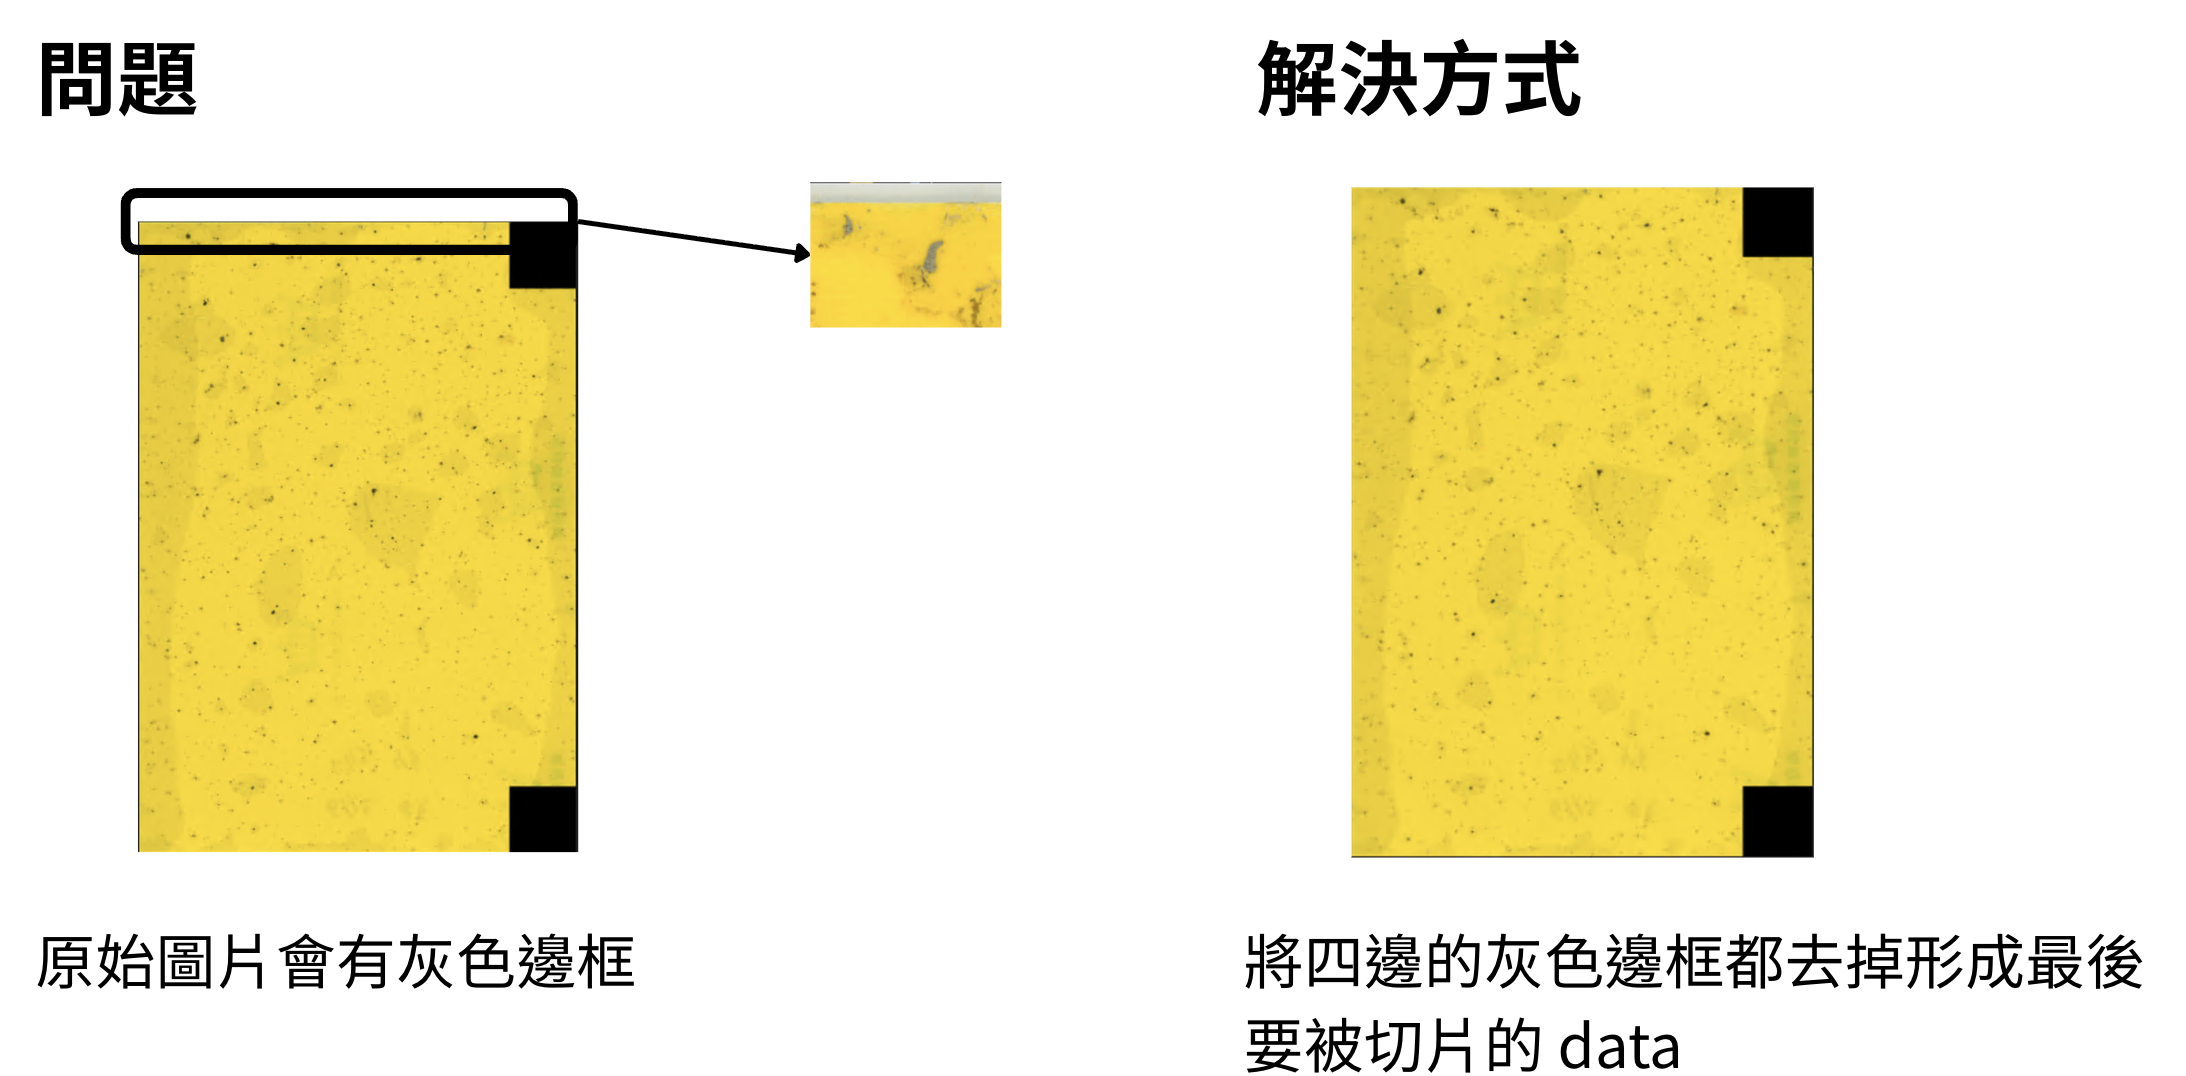
\includegraphics[width=0.45\linewidth]{preprocess_corners.png}
  \caption{Preprocessing. Left: removing the gray frame keeps only the active yellow trap area. Right: blackening the punched-hole regions prevents them from being mistaken for insects in the next stage.}
  \label{fig:preprocess}
\end{figure}

\begin{figure*}[t]
  \centering
  
\includegraphics[width=0.95\textwidth]{adaptive_tile_diagram.png}
  \caption{Four-step adaptive tiling: (1) probe-tile scan; (2) HSV-based foreground detection (yellow $+$ black ratio $<$ \texttt{-{}-yellow-threshold}); (3) merging of adjacent / overlapping tiles into one bounding box; (4) padded crop saved as an independent image.}
  \label{fig:adaptivetile}
\end{figure*}

\begin{figure*}[t]
  \centering
  % Replace with a vector re-render of the README Mermaid diagram.
  \fbox{\parbox{0.9\textwidth}{\centering \textit{[Pipeline figure --- re-render the README Mermaid flowchart as a vector image and place it here.]}\\[1ex] \texttt{raw $\rightarrow$ preprocess $\rightarrow$ training (DINOv2 $+$ SeCu $+$ medoid $+$ MML) $\rightarrow$ inference $\rightarrow$ sub-clustering}}}
  \caption{End-to-end system pipeline. Raw board photographs are cleaned and tiled into single-insect crops, the SeCu model is trained on these crops, every crop is assigned to a coarse cluster at inference, and the optional sub-clustering stage refines a coarse cluster into finer groups.}
  \label{fig:pipeline}
\end{figure*}

\begin{figure*}[t]
  \centering
  \begin{tabular}{cccc}
    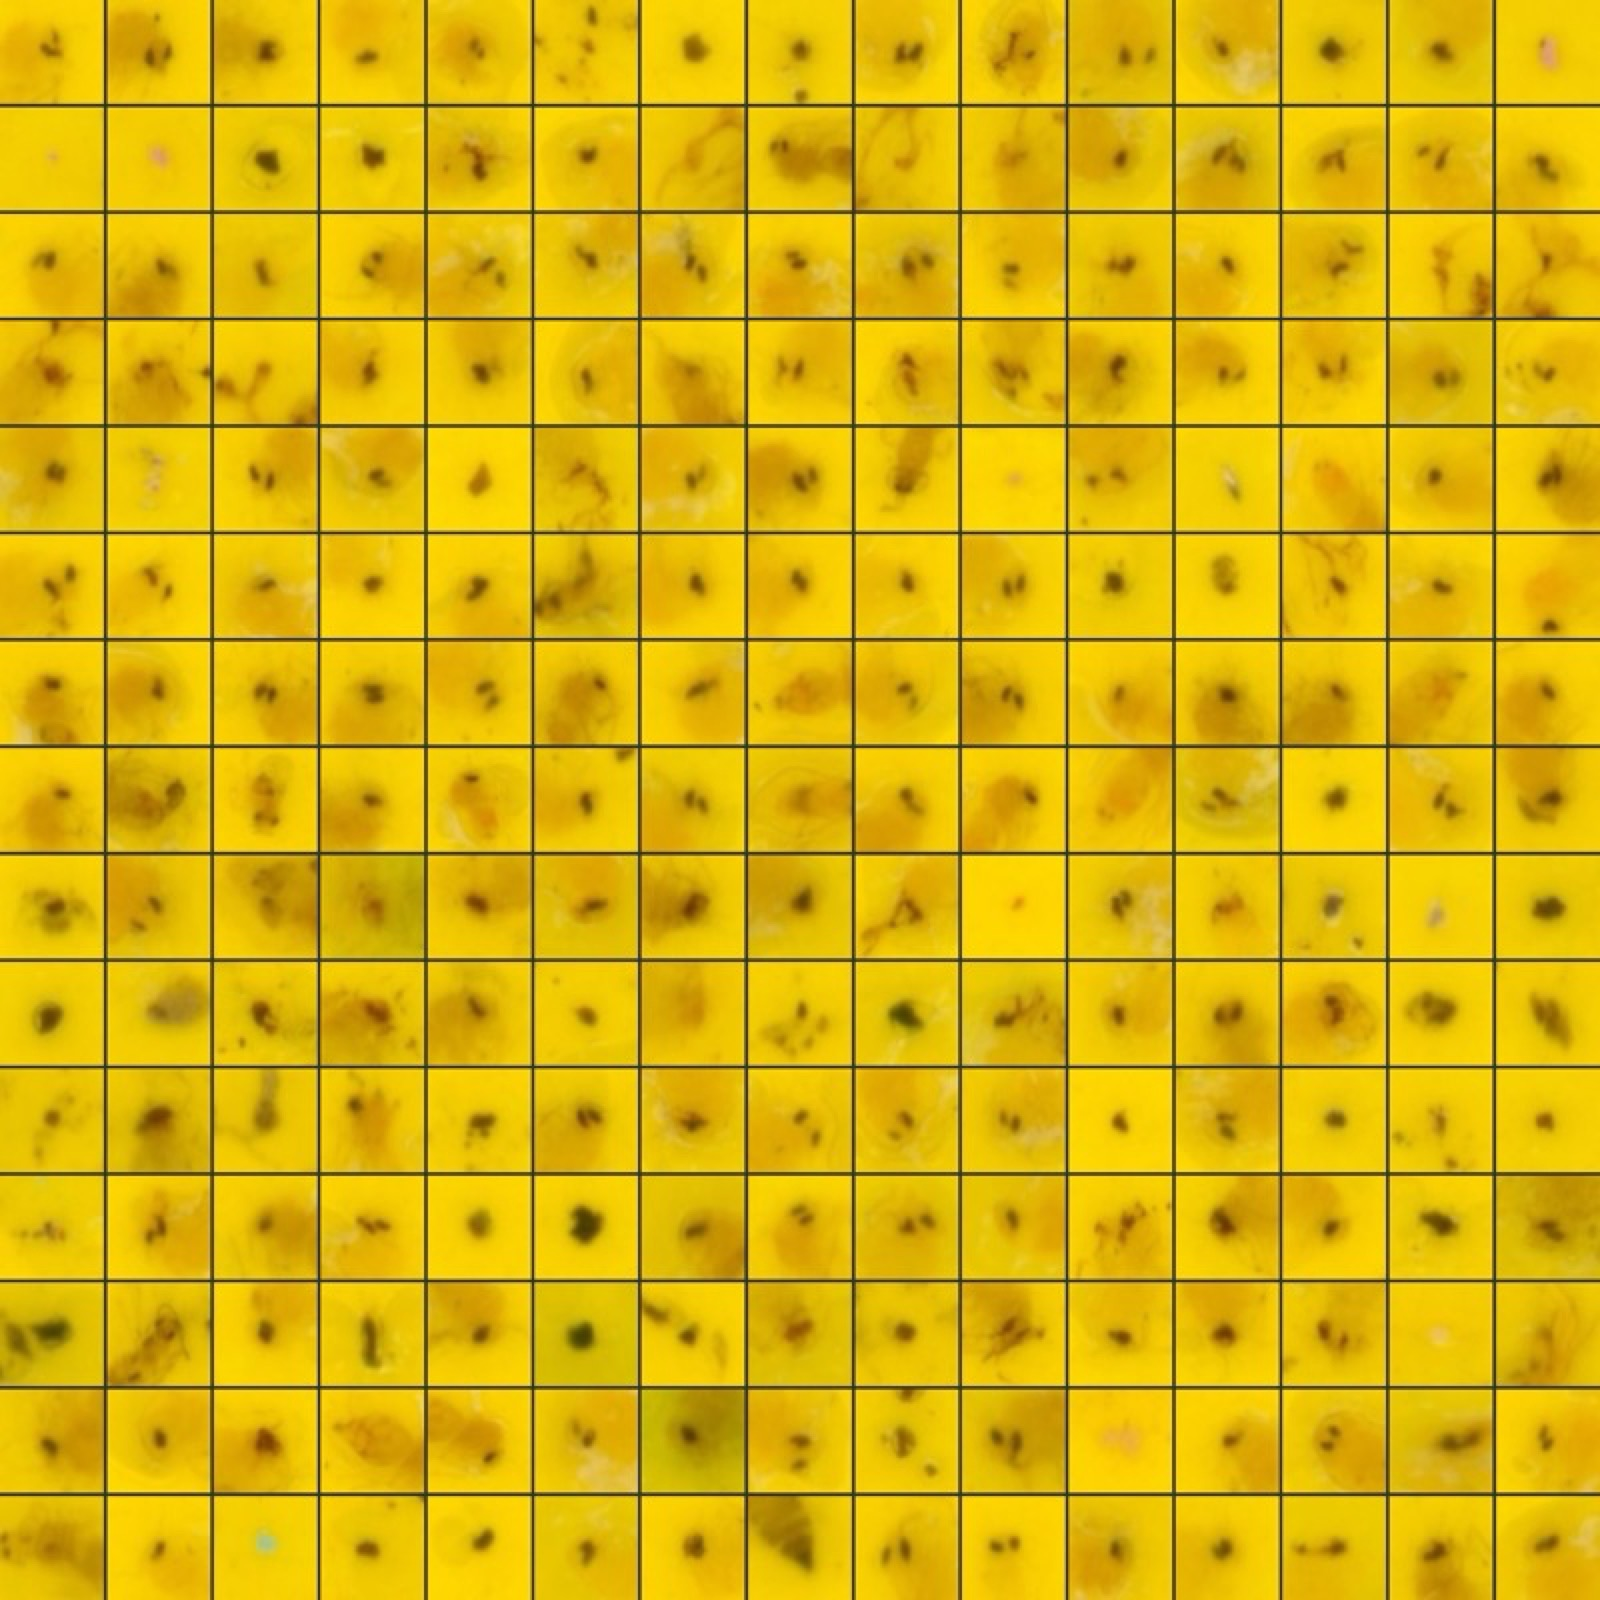
\includegraphics[width=0.22\textwidth]{cluster_0.jpg} &
    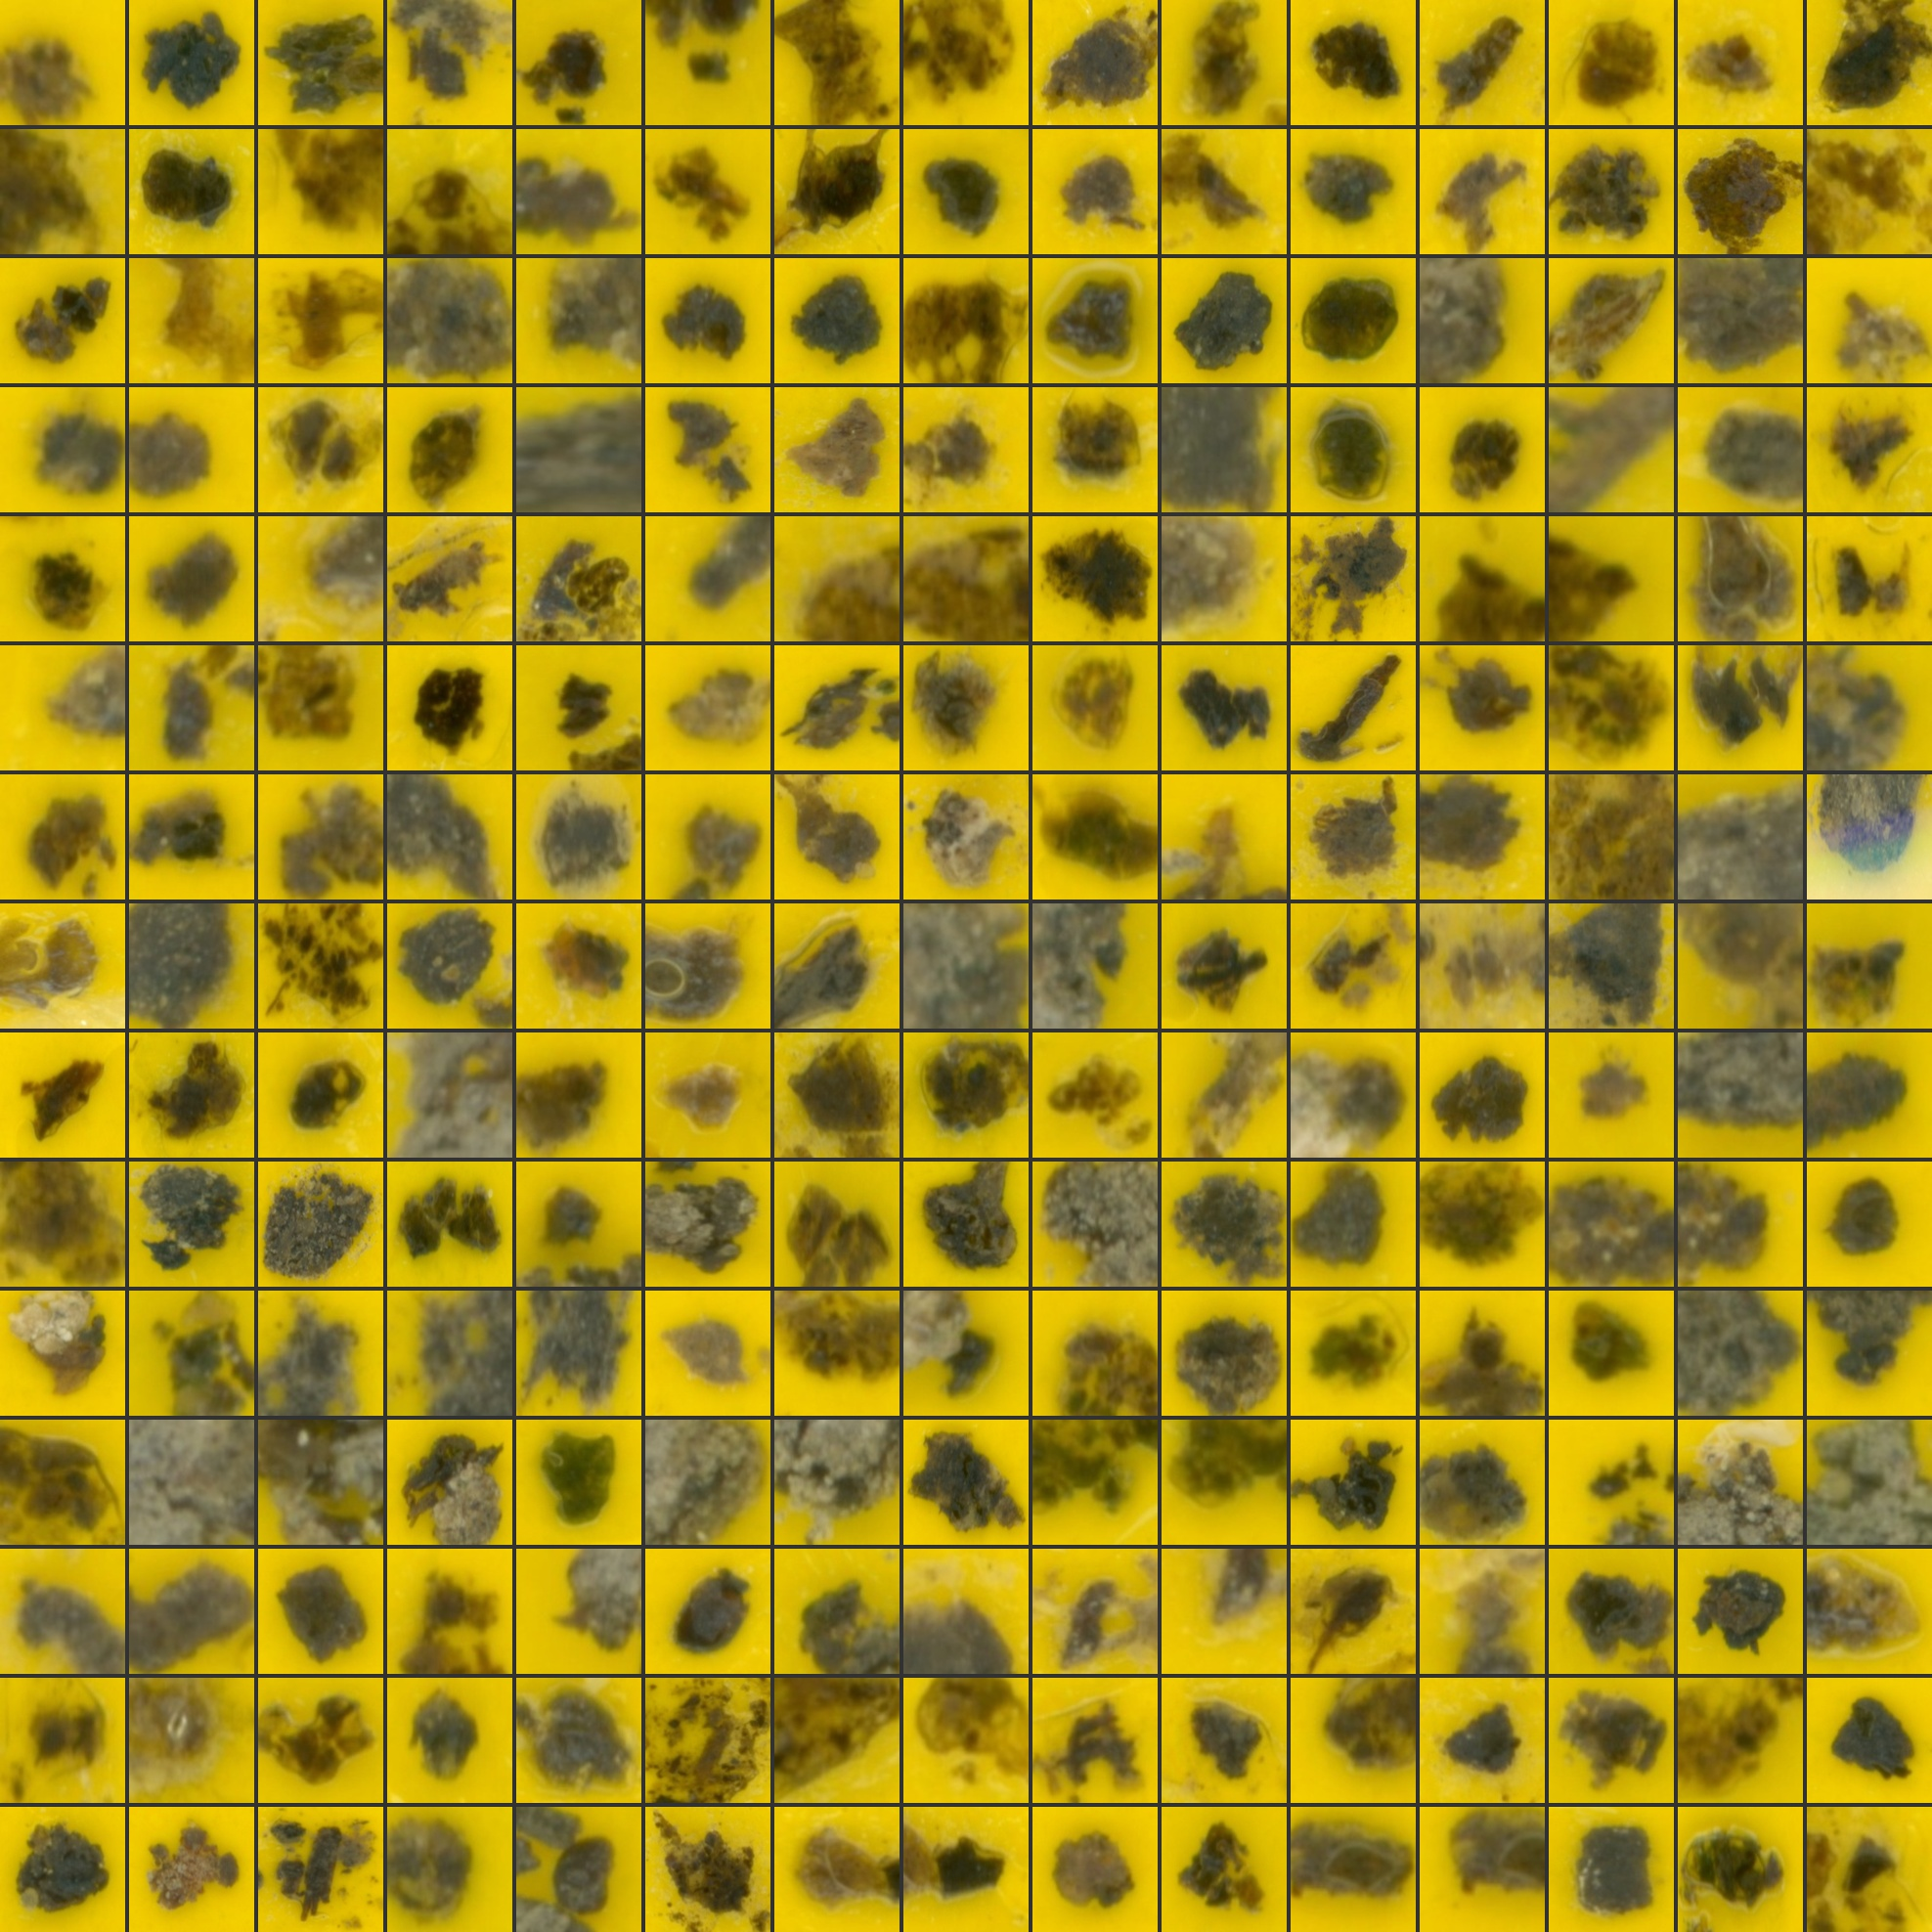
\includegraphics[width=0.22\textwidth]{cluster_1.jpg} &
    
\includegraphics[width=0.22\textwidth]{cluster_2.jpg} &
    
\includegraphics[width=0.22\textwidth]{cluster_3.jpg} \\
    \small Cluster 0 & \small Cluster 1 & \small Cluster 2 & \small Cluster 3 \\
    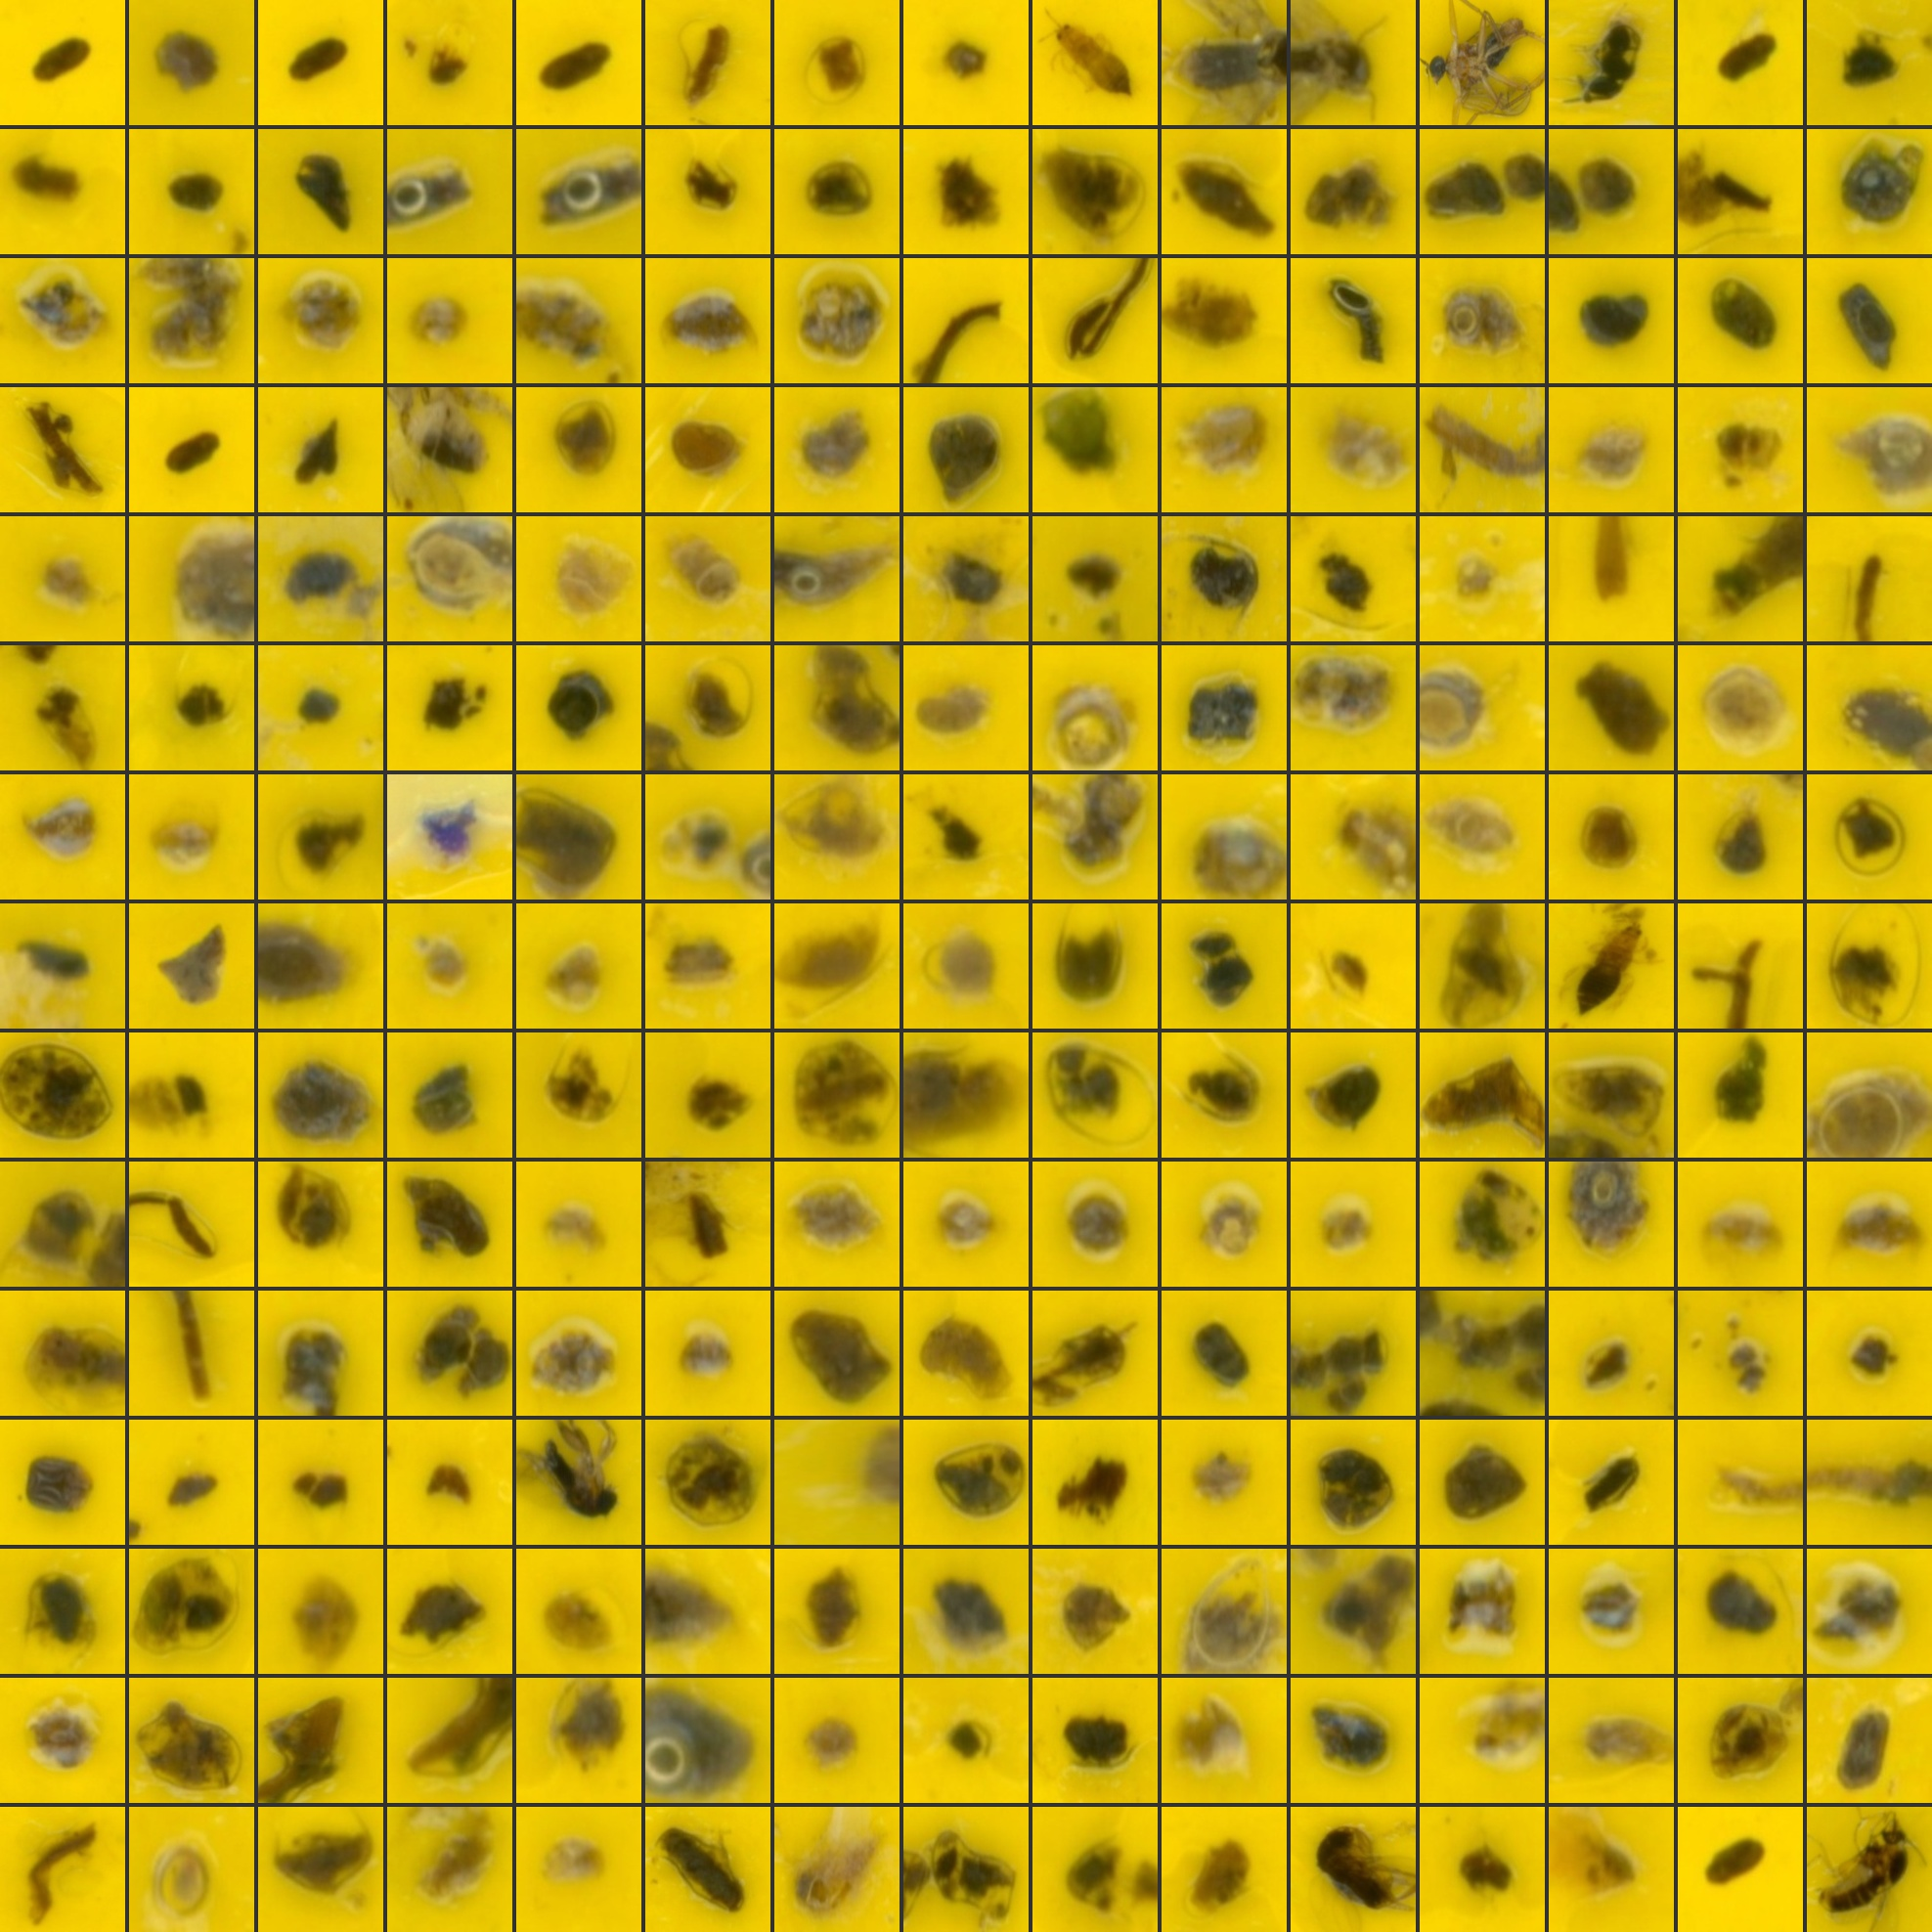
\includegraphics[width=0.22\textwidth]{cluster_4.jpg} &
    
\includegraphics[width=0.22\textwidth]{cluster_5.jpg} &
    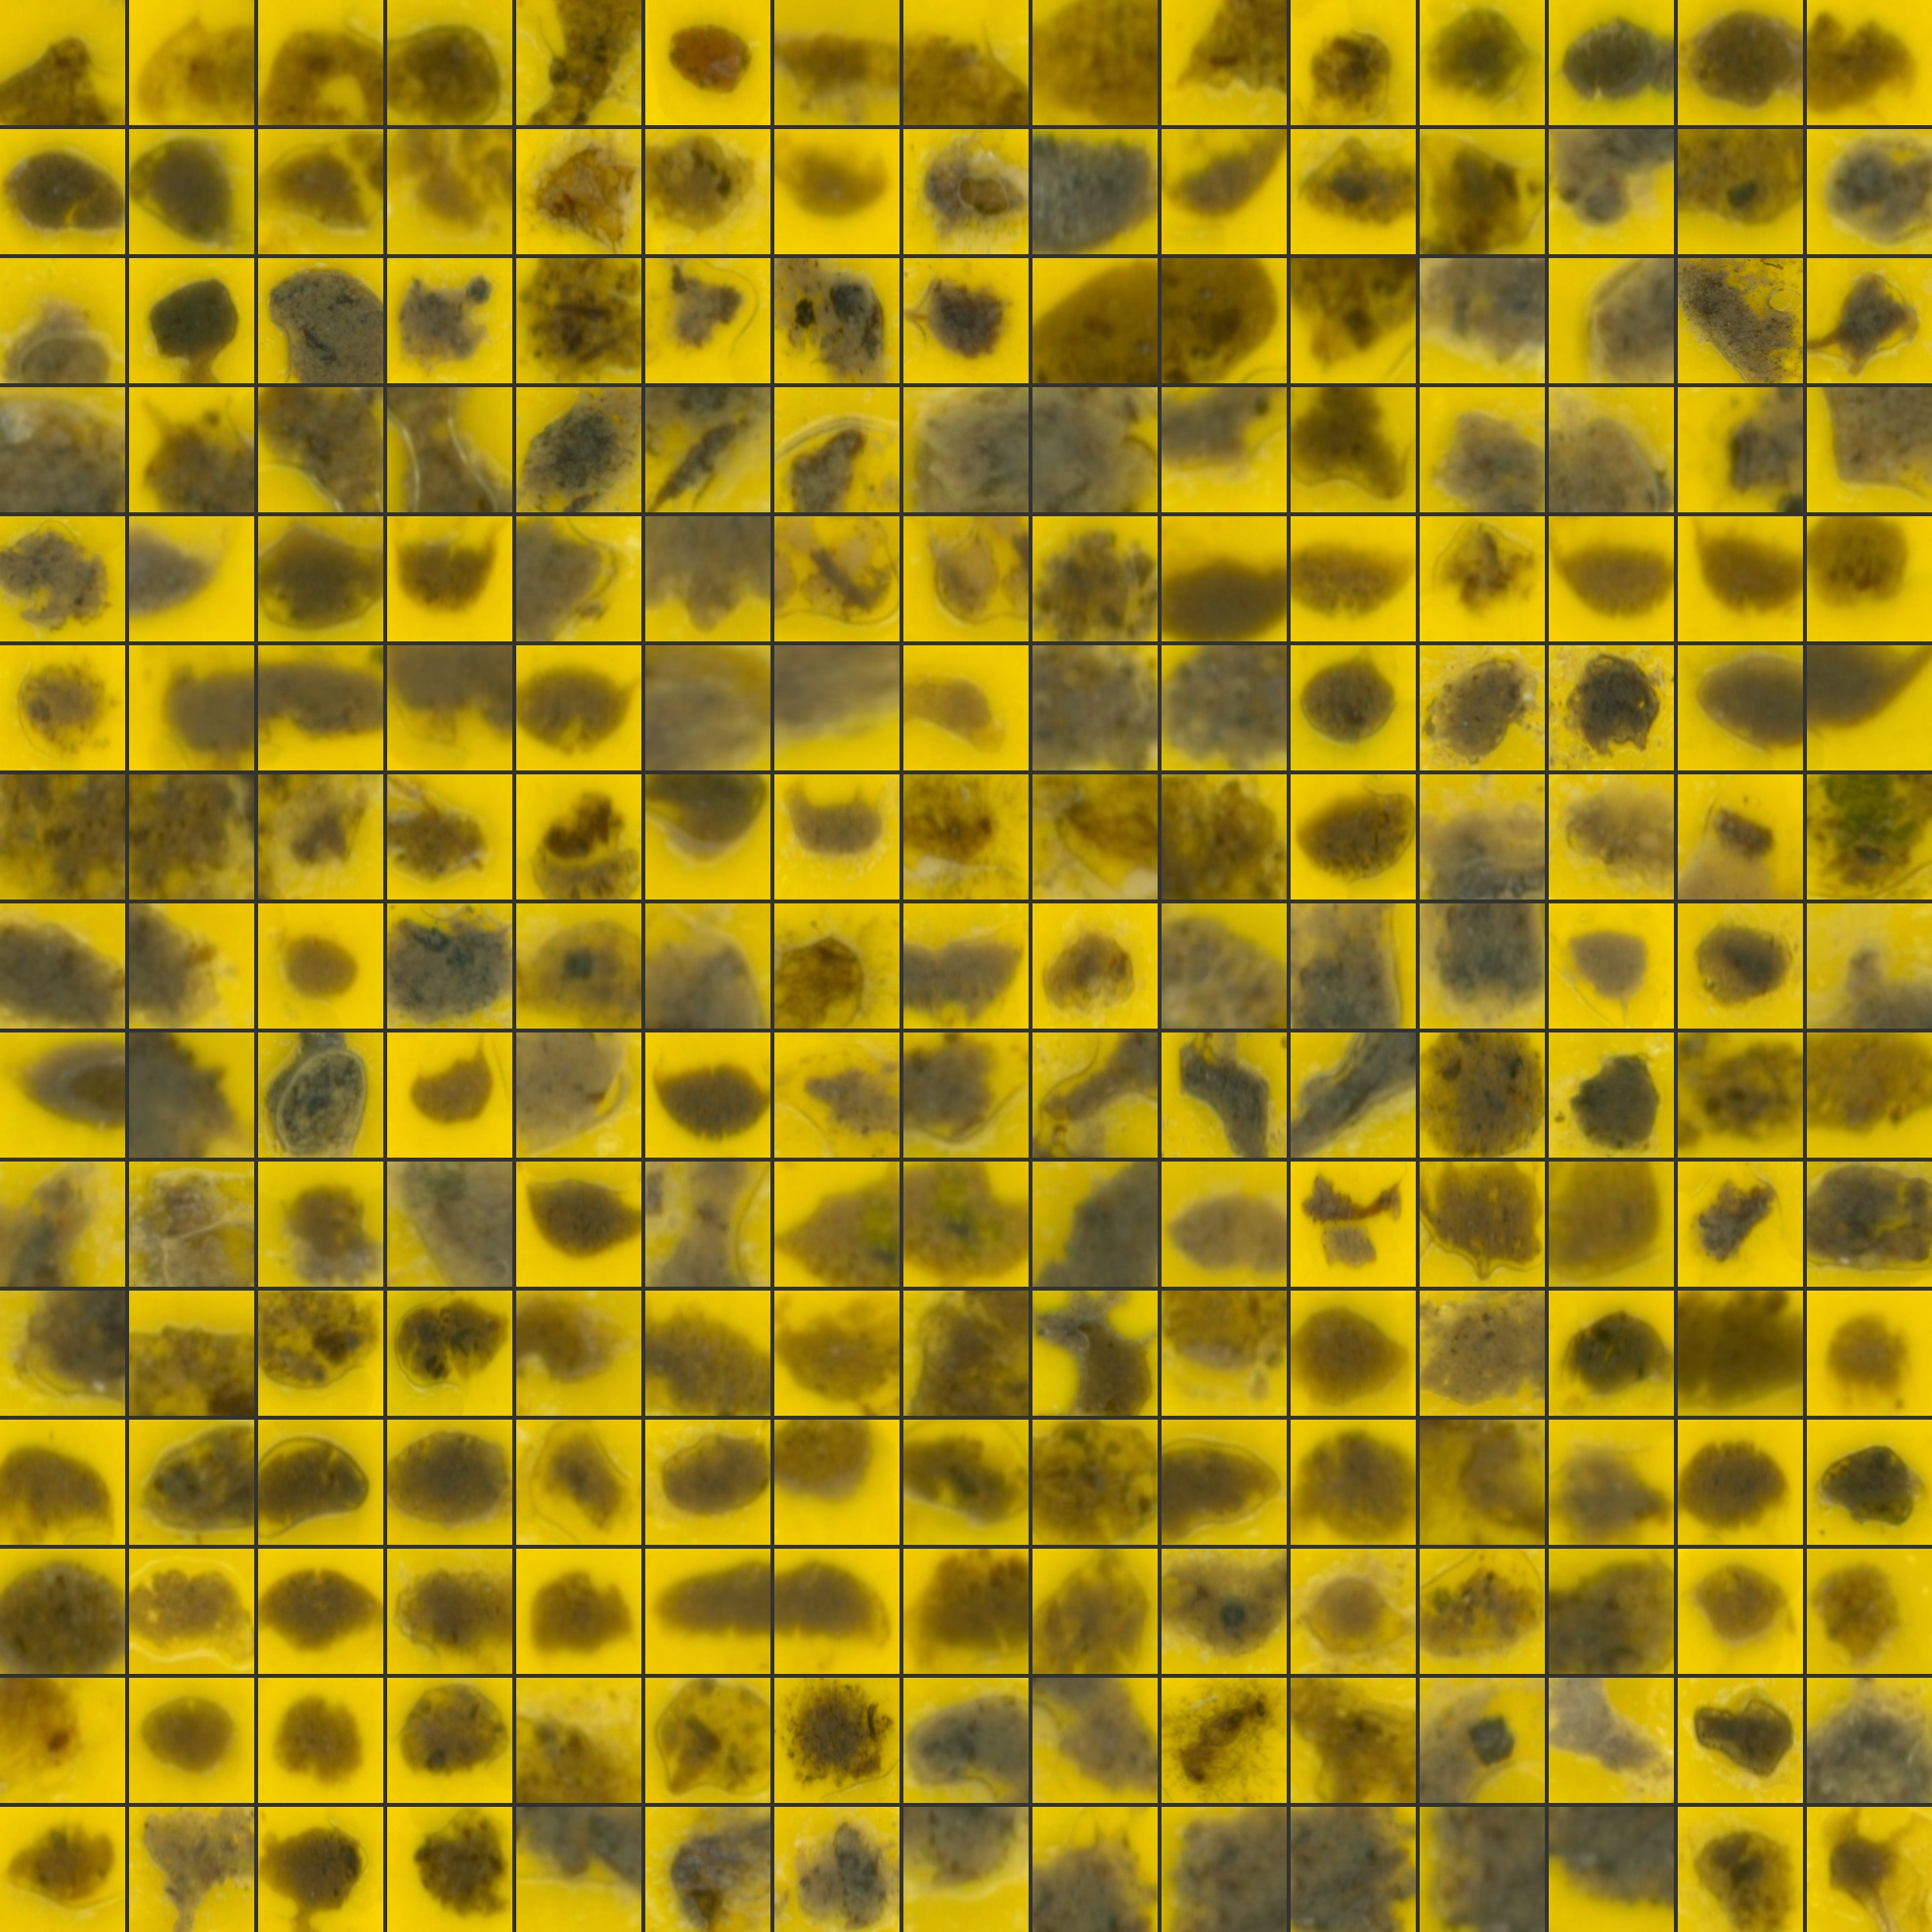
\includegraphics[width=0.22\textwidth]{cluster_6.jpg} &
    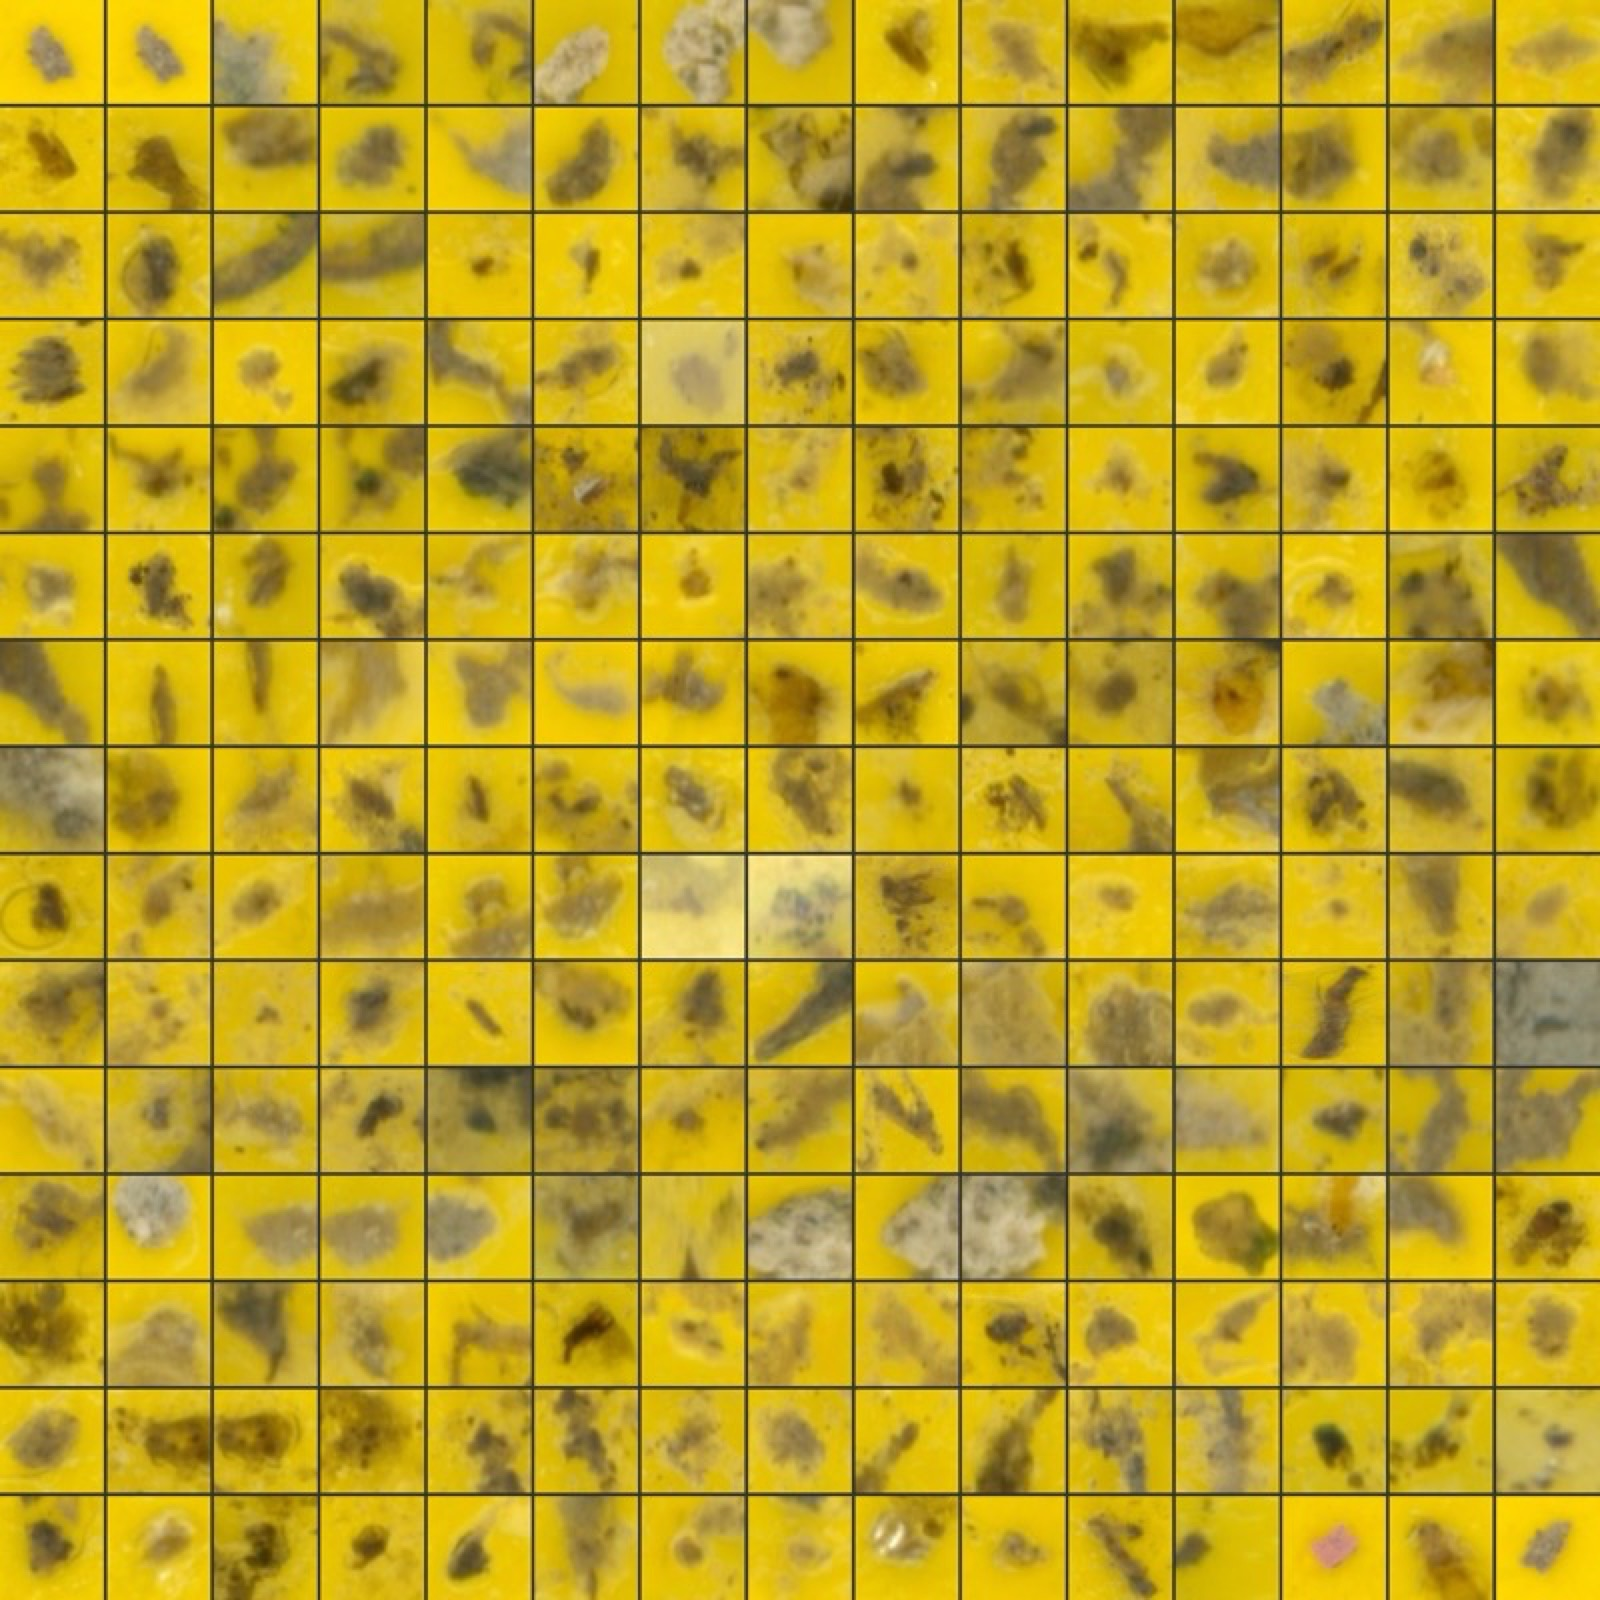
\includegraphics[width=0.22\textwidth]{cluster_7.jpg} \\
    \small Cluster 4 & \small Cluster 5 & \small Cluster 6 & \small Cluster 7 \\
  \end{tabular}
  \caption{Representative crops from the eight coarse clusters obtained with DINOv2 $+$ SeCu $+$ MML on $4{,}305$ greenhouse insect crops. Within each cluster, samples share a consistent body shape, color, and size.}
  \label{fig:clusters}
\end{figure*}

\begin{figure}[t]
  \centering
  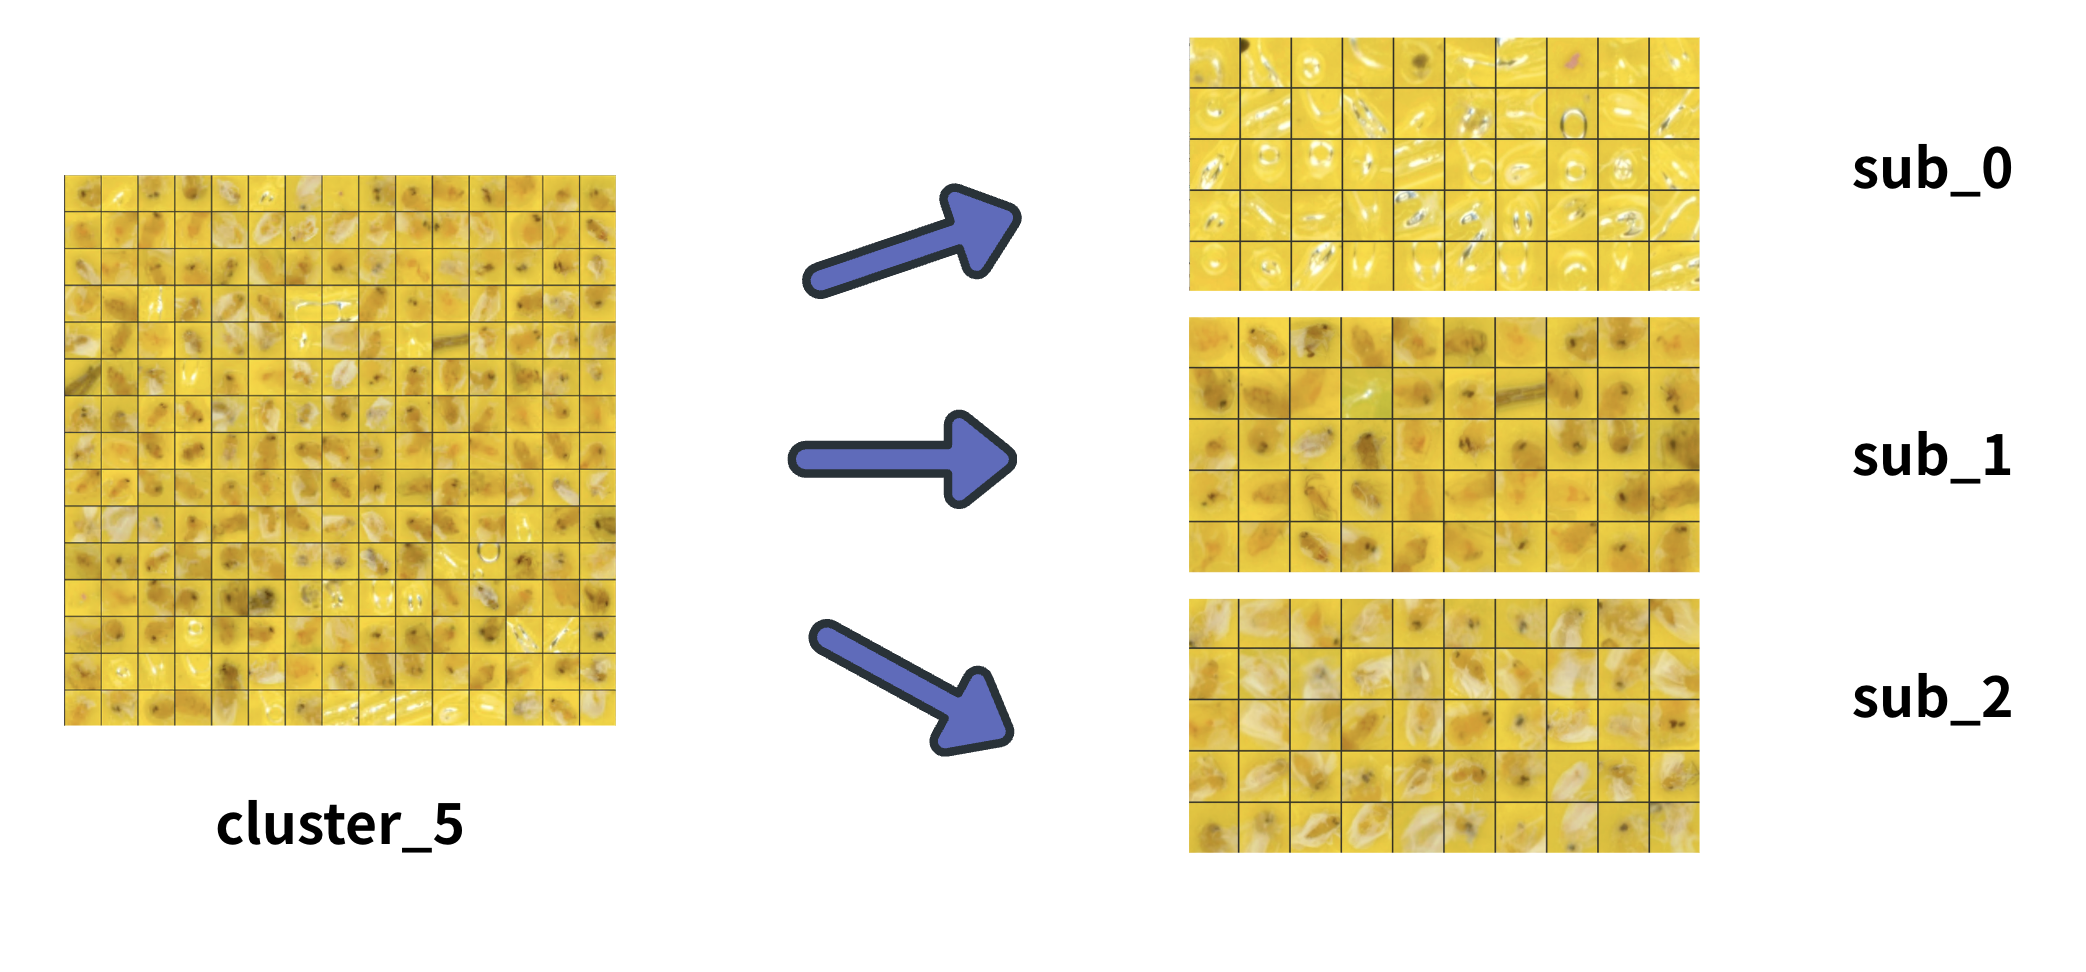
\includegraphics[width=0.95\linewidth]{subcluster_example.png}
  \caption{Hierarchical sub-clustering on a single coarse cluster. The mixed coarse cluster (top) is split into cleaner sub-groups (bottom) by the ensemble HDBSCAN stage, with low-stability samples isolated as ``uncertain.''}
  \label{fig:subcluster}
\end{figure}

\begin{figure}[t]
  \centering
  % Replace with the latest 3-D t-SNE PNG from Secu-revised/output/
  \fbox{\parbox{0.9\linewidth}{\centering \textit{[3-D t-SNE PNG --- drop in the latest output from Secu-revised/output/]}}}
  \caption{3-D t-SNE visualization of the learned embedding for the eight coarse clusters. Distinct colored regions correspond to the eight clusters; well-separated regions indicate that the unsupervised representation captures meaningful morphological differences.}
  \label{fig:tsne}
\end{figure}

\end{document}
